%=========================================================================
% (c) 2011, 2012 Josef Lusticky

\chapter{Hardware real-time support}
\begin{figure}
	\centering
	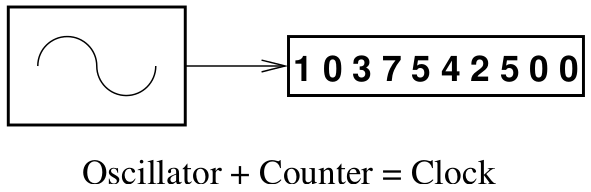
\includegraphics[width=6cm,keepaspectratio]{fig/clock.png}
	\caption{Clock by P. Kamp}
	\label{fig:hw-clock}
	%\bigskip
\end{figure}
For keeping, measuring and resolving time computer needs a clock.
Computer clock is an electronic device that counts oscillations in a
quartz crystal oscillator with a particular frequency~\cite{thesis-sync}.
These clocks are essentially timers associated with a counter register and
are capable of generating hardware interrupts.
The counter register counts the oscillations of the crystal.
When the counter registers reaches a specific value,
an interrupt is generated.
Such interrupt is called a {\it{clock tick}} (or {\it{timer tick}}) and at each clock tick,
interrupt service routine increments a system clock value stored in memory~\cite{thesis-sync}.

\section{Time handling}
In a typical computer clock design, interrupts are produced at
fixed tick intervals in the range 1-20~ms~\cite{nanokernel}.

A typical desktop computer today includes CPU based on Intel x86 architecture.
Real-Time Clock (RTC) in CMOS memory that is battery powered

Therefore a usual process of time handling
used by first Unix-like operating systems on x86 architecture
was as follows.
The kernel read the current time from RTC and stored its value in memory during boot.

Starting with Intel 386, Intel introduced
Programmable Interrupt Controller (PIT) Intel 8253 and 8254 - 3 counters (counter 0 interrupt to OS)

Used by historic versions of Linux
=> read initial time from RTC, setup PIT and interrupts (IRQ 0, INT 8), increment jiffies on every interrupt, provide application resolution of jiffies

init/main.c - time\_init() - read from RTC and save to startup\_time
kernel/sched.c - sched\_init() = PTI setup for interrupts - LATCH (1193180/HZ)
kernel/system\_call.s - timer\_interrupt() in assembly - increments jiffies

The current real time is provided by CURRENT\_TIME (startup\_time+jiffies/HZ) => since jiffies is integer and HZ is 100 => resolution of 10ms.
kernel/sys.c - sys\_time() - CURRENT\_TIME returned

Unfortunately Intel x86 architecture is heavily influenced by backward compatibility,
and many hardware configurations are in use today -
e.g. the time value can also be stored in Binary Code Digit (BCD) encoding in RTC.

and there are many possible hardware configurations among these computers today.
HPET, ... %nasleduje TODO-...

TICK - http://www.ntp.org/ntpfaq/NTP-s-sw-clocks-tick.htm


- software:
The Kernel Discipline =  kernel clock model RFC 1589

However, some clock implementations do not allow small corrections to be applied to the system clock, and there is no standard interface to monitor the system clock's quality.
=> divide problem (in RFC)

%FROM HERE DONE
In recent years, a new design called {\it{tickless}} or {\it{dynamic ticks}}
has been in development~\cite{kernel-timer-systems}.
This allows an operating system kernel to run without a regular timer tick.
Such design is not used by Contiki OS~\cite{contiki-docs} and
therefore not further discussed in this thesis.

\section{Clock quality factors}
Unfortunately all the common clock hardware is not very accurate.
This is simply because the frequency that makes time increase is never exactly right.
Even an error of only 0.001\% would make a clock be off by almost one second per day~\cite{ntp-faq}.
Almost every clock can have an unique behaviour depending on many conditions.
The following factors are therefore used for expressing clock quality and behaviour:
\begin{itemize}
\item
Frequency is the rate at which a clock progresses~\cite{thesis-sync}.
\item
It is sometimes convenient
to express frequency offsets in parts-per-million~(PPM), where~1~PPM
is equal to $10^{-6}$ $\frac{s}{s}$ (0.0001\%)~\cite{rfc5905}.
\item
From long-term observation one may also notice variations in the clock frequency.
The difference of the frequency is called wander~\cite{ntp-faq}.
There can be clocks with poor short-term stability, but with good long-term stability, and vice versa.
\item
Resolution is the smallest possible increase of time the clock model allows.
If a clock increments its value only once per second, its resolution is also one second~\cite{ntp-faq}.
\item
Precision is the smallest possible increase of time that can be experienced
by a program~\cite{ntp-faq}.
\item
When repeatedly reading the time, the difference may vary almost randomly.
The difference of these differences (second derivation) is called jitter~\cite{ntp-faq}.
\item
Accuracy determines how close is the clock to an official time reference~\cite{ntp-faq}.
\item
Offset is the difference between the time read by the clock and the reference time~\cite{thesis-sync}.
\item
Reliability determines the time a clock can keep within a specified accuracy~\cite{ntp-faq}.
\end{itemize}

As mentioned before, all of the common hardware clock is not very accurate.
Real clocks have a frequency error of several PPM quite frequently
and some of the best clocks available still have errors of about $1^{-8}$PPM~\cite{ntp-faq}.
Even if the systematic error of some clock model is known, the clock will never be perfect.
This is because the frequency varies over time, mostly influenced by temperature,
but it could also be air pressure or magnetic fields~\cite{ntp-faq}.

For keeping an accurate time a clock not only needs to be read, it must be also set.
However, simply setting the clock to remove the offset would cause unpredictable time steps.
Since time is an always monotonically increasing function, this is not a desired behaviour.
Minimising the time offset and frequency difference between
the reference clock and the local clock without any time step
is one of the main goals of Network Time Protocol and its algorithms.
